% !TEX encoding = UTF-8 Unicode
% !TEX root = thesis-ex.tex

This discussion is based on the model introduced in Ref. \cite{Spousta:2015fca}. This phenomenological model emphasizes the jet \pt\ dependence of the quark to gluon fraction and the difference between quark-jet and gluon-jet quenching. It uses an ``extended'' power law parameterization of the high-\pt\ hadron spectra coupled with a quenching that is based on a non-constant fractional energy loss. This model considers the different color charges carried by quarks and gluons and their different splitting functions, and assumes that gluon jets lose energy at a rate 9/4 times higher than quark jets. The key assumption of the model are:
\begin{itemize}
\item The energy lost by a jet is radiated at large angles and does not appear within the jet cone. This is backed by \cite{Chatrchyan:2011sx}.
\item The fragmentation pattern of the jet is unaffected by the presence of the QGP i.e. they fragment as they would in a vacuum. This is motivated by the idea that the QGP is unable to resolve the internal jet structure and is supported by \cite{Blaizot:2013hx, CasalderreySolana:2012ef}.
\end{itemize} 

The model uses the following extended power-law parameterization to describe the high-\pt\ jet spectra:

\begin{align}
\frac{dn}{d\ptjet} = A \left( \frac{\pt_0}{\ptjet} \right) ^{n+\beta \log(\ptjet / \pt_0)}
\end{align}

where $\pt_0$ is a reference transverse momentum at which $A= dn/d\ptjet$, $\beta$ is the logarithmic derivative of $dn/d\ptjet$ at $\ptjet = \pt_0$. Then considering the different quark and gluon fractions as $f_{q0}$ and $f_{g0} = 1-f_{q0}$ respectively, the combined spectrum for quarks and gluons can be written as:

\begin{align}
 \frac{dN}{d\ptjet} &= A \left[ f_{q0} \left( \frac{\pt_0}{\ptjet} \right)^{n_q+ \beta_q \log(\ptjet / \pt_0)} + (1-f_{q0}) \left( \frac{\pt_0}{\ptjet} \right)^{n_g + \beta_g \log(\ptjet / \pt_0)} \right] \\
\nonumber \\ 
\label{eq:eq_q_frac} f_q (\ptjet) &= \dfrac{1}{1 + \left(\dfrac{1-f_{q0}}{f_{q0}}\right) \left( \dfrac{\pt_0}{\ptjet}\right)^{\Delta n + \Delta \beta \log(\ptjet/\pt_0)} }
\end{align}
where $\Delta n = n_g - n_q$ and $\Delta \beta = \beta_g - \beta_q$. The \pt\ dependence of the quark fraction along with the fit is shown in Figure~\ref{fig:raa_centDep}. The fragmentation functions can also be determined using final-state charged hadrons within a $R=0.4$ jet cone. These are fit to the form \Dz, with fits for the quark and gluon fragmentation shown in Figure~\ref{fig:gluon_fragmentation}.


\begin{align}
D(z) = a \times \frac{(1+dz)^b}{(1+ez)^c} \times e^{-fz}
\label{eq:ff_param}
\end{align}


\begin{figure}
\begin{subfigure}{.45\textwidth}
  \centering
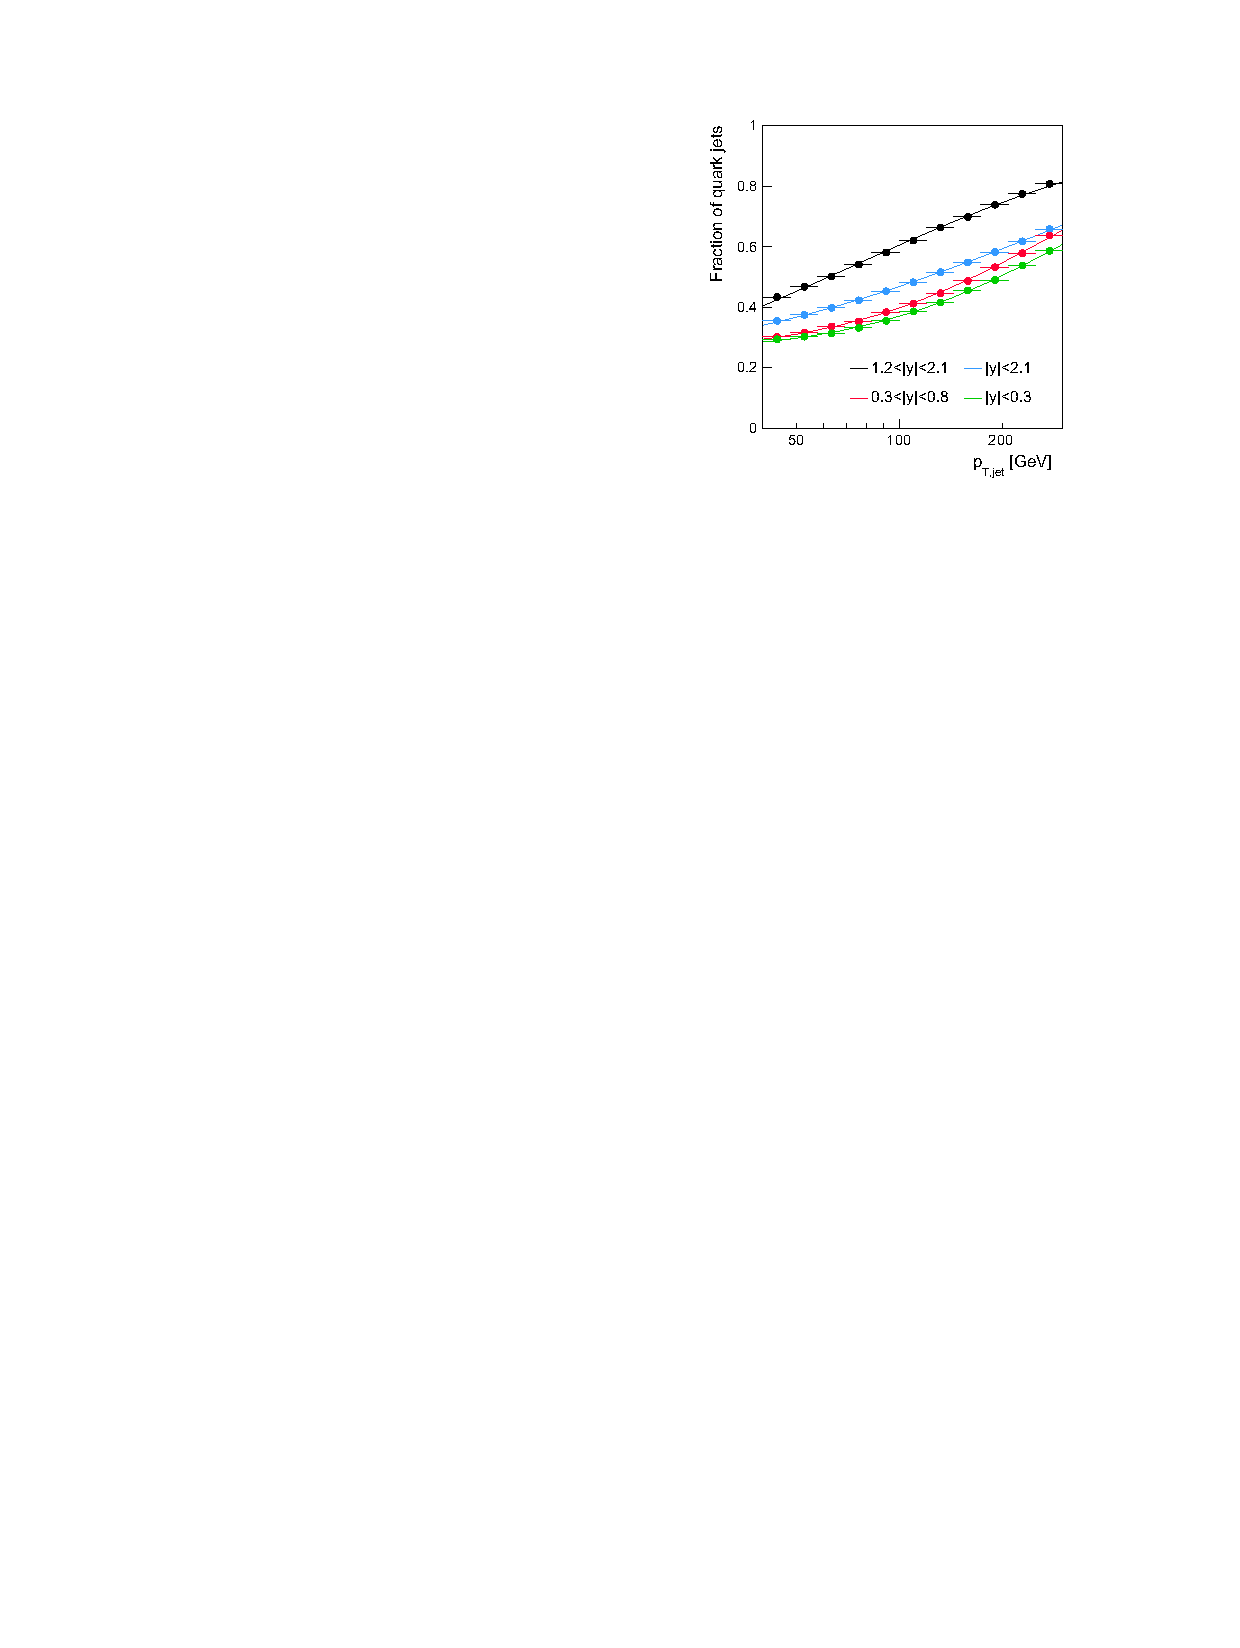
\includegraphics[width=0.8\textwidth]{figures/jetMeasurements/jetQuarkFraction}
\caption{The jet quark fraction as a function of \ptjet\ in different rapidity bins. The points are from \pythia8 simulations and the lines are fits to Equation~\ref{eq:eq_q_frac}.}
\label{fig:raa_centDep}
\end{subfigure} \qquad
\begin{subfigure}{.45\textwidth}
  \centering
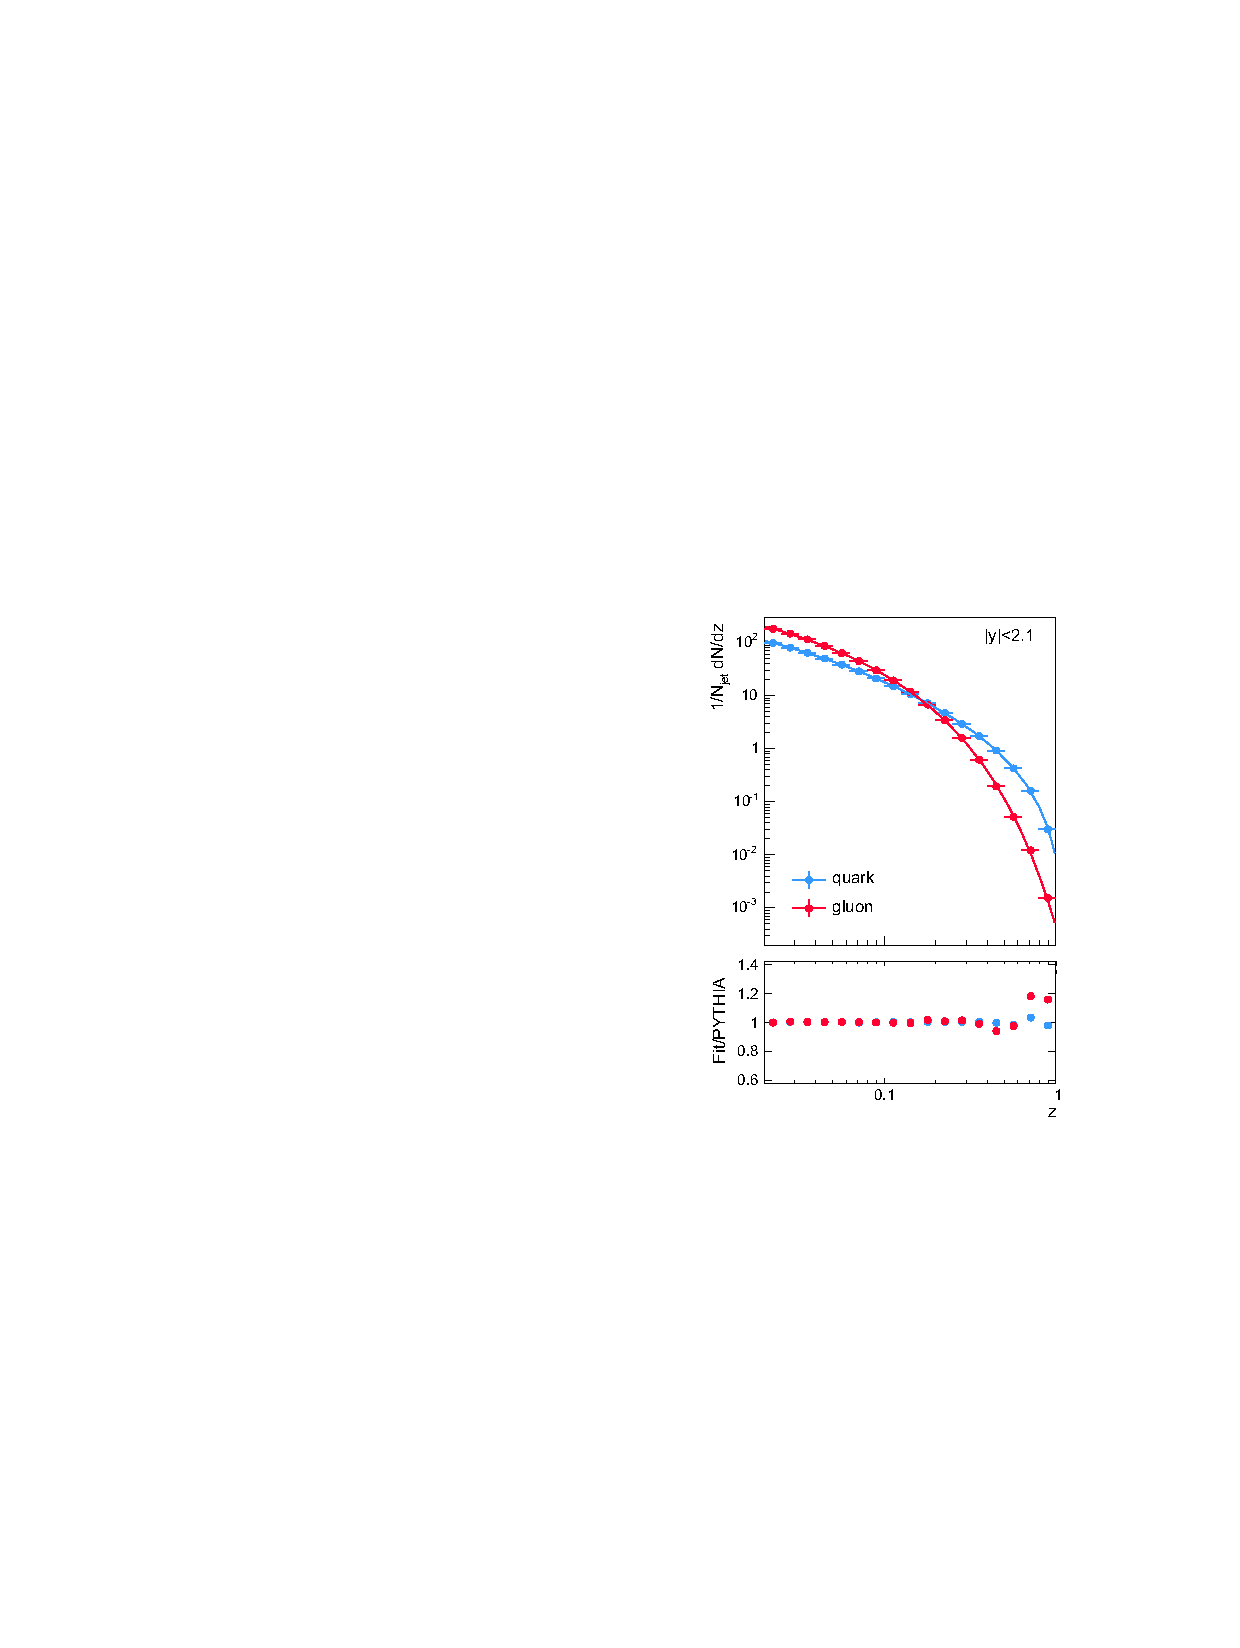
\includegraphics[width=0.8\textwidth]{figures/jetMeasurements/gluon_fragmentation}
\caption{A comparison of the \pythia8 quark and gluon fragmentation. The solid lines are the fits from The jet quark fraction as a function of \ptjet\ in different rapidity bins. The points are from \pythia8 simulations and the lines are fits to Equation~\ref{eq:ff_param}.}
\label{fig:gluon_fragmentation}
\end{subfigure}
\caption{Fits to quark fractions and fragmentation functions from \pythia8.  Figure taken from \cite{Spousta:2015fca}}
\label{fig:EQ_pp_models}
\end{figure}


For the quenched spectra, this model assumes a non-constant fractional shift given below as $S$. This approach is based on \cite{baier2001quenching} and is used because of the inability of the constant fractional shift to explain the jet \pt\ dependence of measured \RAA. 

\begin{align}
S = s' \left( \frac{\ptjet}{\pt_0} \right) ^\alpha
\end{align}
where $\alpha$ is an undetermined parameter and $s'$ is the shift for a jet with $\ptjet = \pt_0$. This gives the following quenched high-\pt\ hadron spectra:

\begin{align}
 \frac{dN_Q}{d\ptjet} &= A \Bigg[ f_{q0} \left( \frac{\pt_0}{\ptjet+S_q} \right)^{n_q+ \beta_q \log\big((\ptjet+S_q) / \pt_0\big)} \left(1 + \frac{dS_q}{d\ptjet} \right) \\
& + (1-f_{q0}) \left( \frac{\pt_0}{\ptjet+S_g} \right)^{n_g + \beta_g \log\big((\ptjet+S_g) / \pt_0\big)}  \left(1 + \frac{dS_g}{d\ptjet} \right) \Bigg] \nonumber
\end{align}
Where the $(1+dS/d\ptjet)$ term is a Jacobian to preserve the number of jets. 
Then the \RAA\ can be written as:

\begin{align}
\RAA = f_q & \left(\frac{1}{1 + S_q / \ptjet}\right) ^{n_q + \beta_q \log\big((\ptjet+S_q)/\pt_0\big)}  \frac{\pt_0}{\ptjet}^{} \left( 1+ \frac{dS_q}{d\ptjet} \right) \times  \\
 (1-f_q) & \left(\frac{1}{1 + S_g / \ptjet}\right) ^{n_g + \beta_g \log\big((\ptjet+S_g)/\pt_0\big)}  \frac{\pt_0}{\ptjet}^{} \left( 1+ \frac{dS_g}{d\ptjet} \right)  \nonumber \\
\end{align}
where the flavor fraction is given by Equation~\ref{eq:eq_q_frac}. These can be fit to the measured ATLAS \RAA\ data as shown in Figure~\ref{fig:EQ_RAA} and the parameters $s'$ and $\alpha$ can be extracted as shown in Figure~\ref{fig:eq_param}. 

\begin{figure}[htbp]
\begin{center}
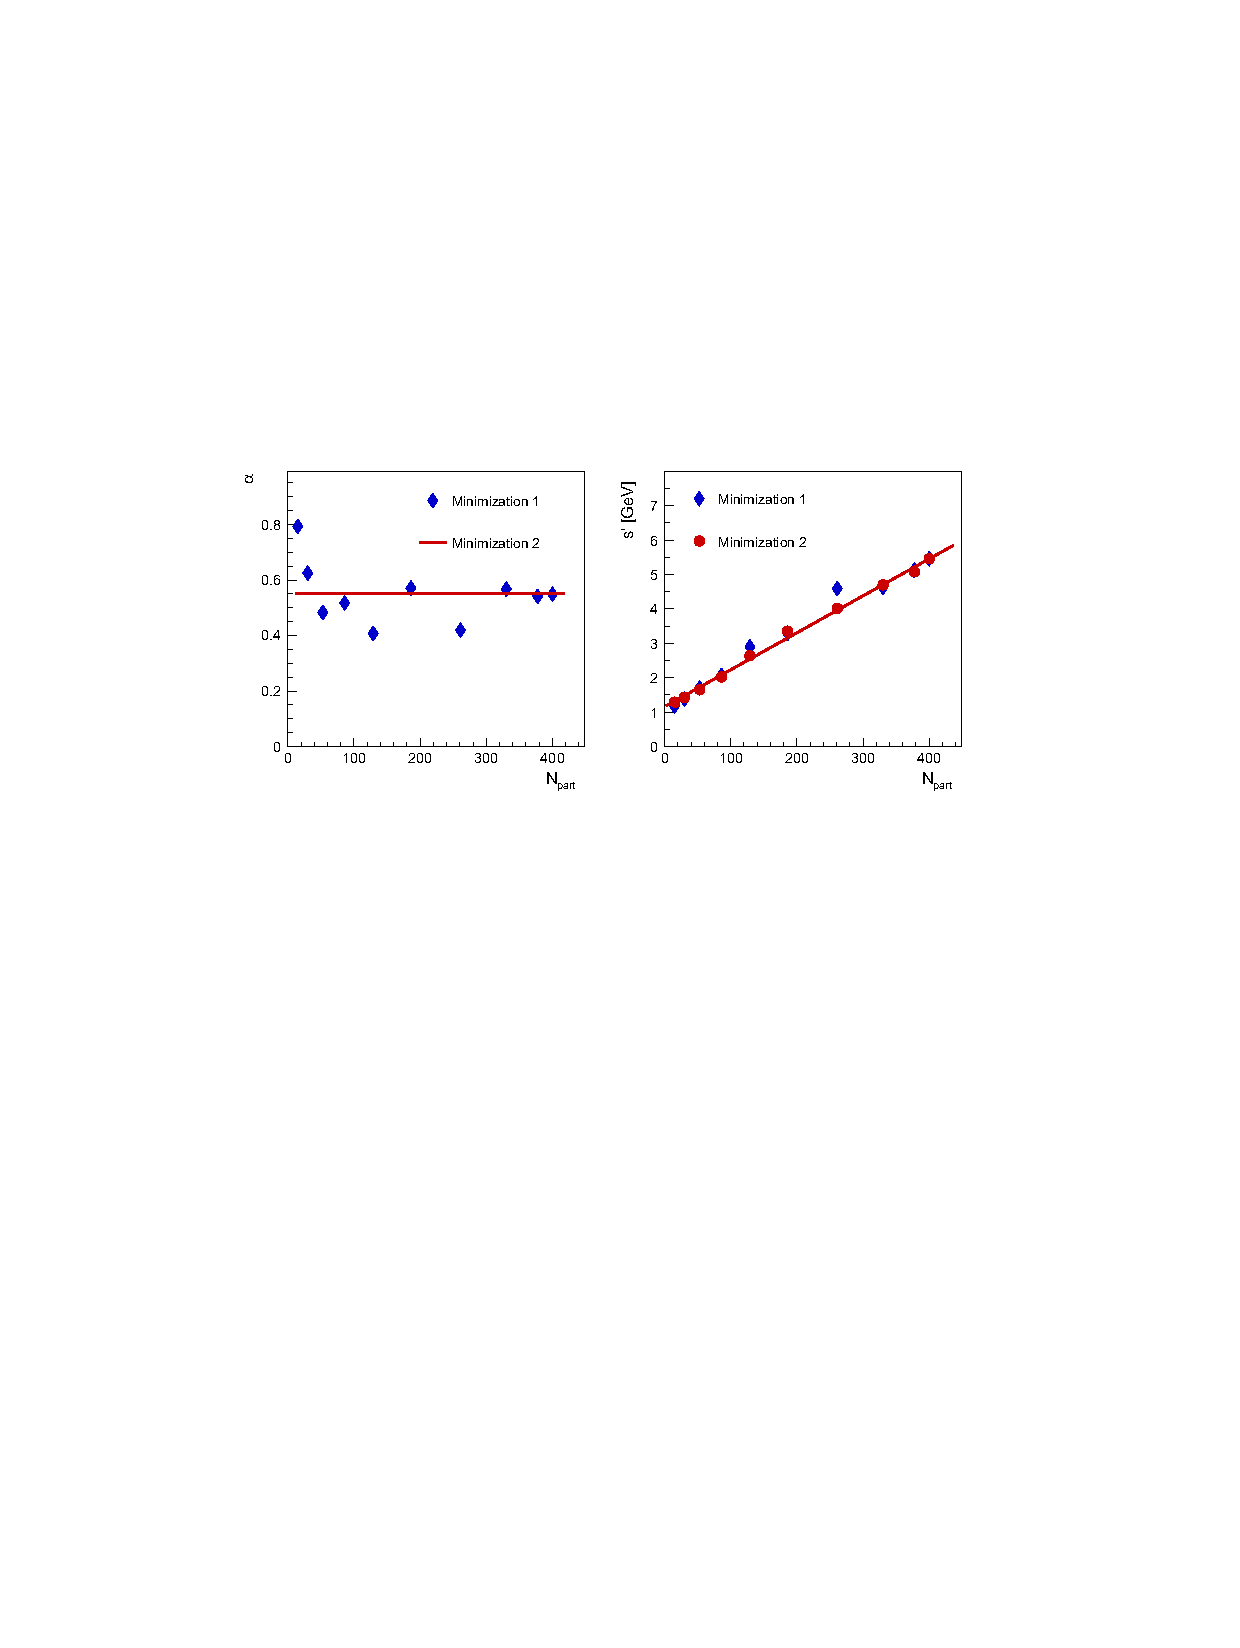
\includegraphics[width=0.55\textwidth]{figures/jetMeasurements/EQ_fitQuality}
\caption{The extracted values of $\alpha$ and $s'$ as a function of \Npart. The first minimization shows fluctuations for $\alpha$ around 0.55, which was then fixed for the second minimization to give an $s'$ that linearly depends on \Npart. Figure taken from \cite{Spousta:2015fca}}
\label{fig:eq_param}
\end{center}
\end{figure}

It can be seen that the analytic fits and the MC are in good agreement. While the fits agree with the data by definition, the robustness of the model can be seen in that it describes the data with a single value for $\alpha$ and a simple centrality dependent shift constant $s'$.  Fits to the \Dz\ distributions are shown in Figure~\ref{fig:EQ_FF} and it can be seen that while the MC and analytic calculation agree well with each other, they are only able to qualitatively capture some features of the data. The enhancement at high $z$ can be explained by an increased quark content of the jet spectrum and subsequent differential quenching for quark and gluon jets. The low $z$ enhancement on the other hand can be considered to be a result of a gluon radiation within the jet or a wake from the medium itself.

\begin{figure}
\begin{subfigure}{1\textwidth}
  \centering
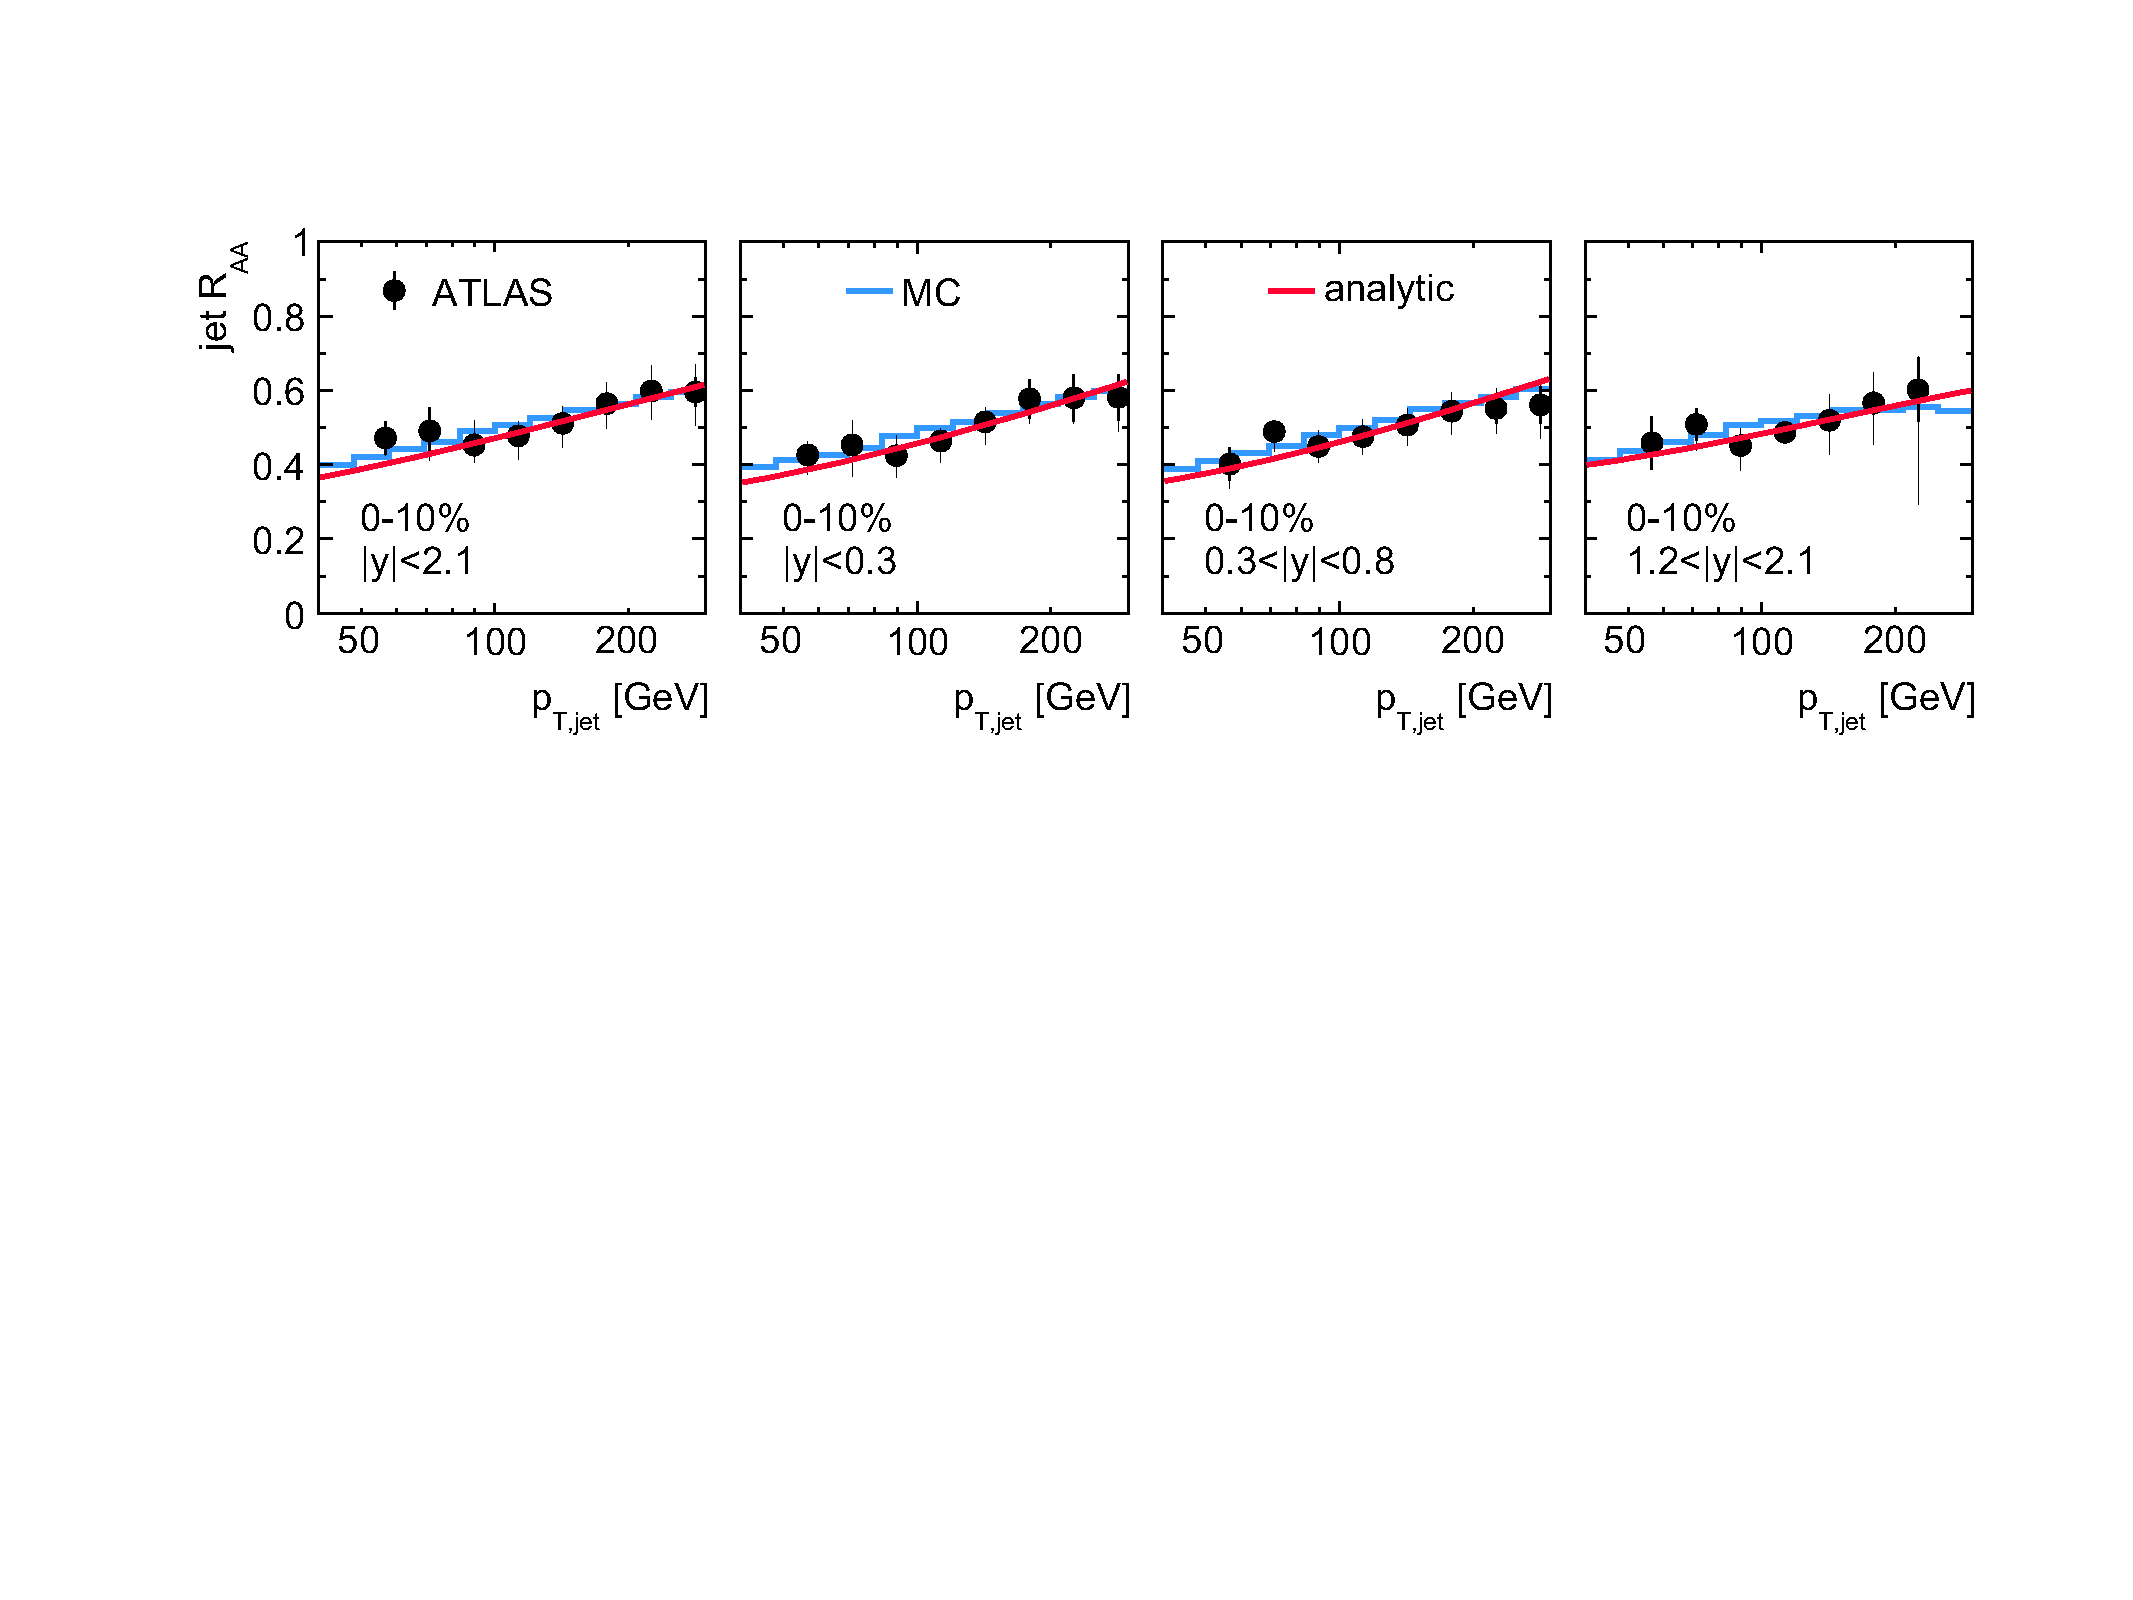
\includegraphics[width=1\textwidth]{figures/jetMeasurements/EQ_RAA}
\caption{A comparison of the \RAA\ as measured by ATLAS for central \pbpb\ collisions in \cite{Aad:2014bxa}, a MC calculation (blue) and the analytic calculation (red) in the EQ model with the extended power-law parameterization and a non-constant fractional energy loss. The different panels are different rapidity intervals.}
\label{fig:EQ_RAA}
\end{subfigure} \\ \\ \\
\begin{subfigure}{1\textwidth}
  \centering
\includegraphics[width=1\textwidth]{figures/jetMeasurements/eq_FF}
\caption{A comparison of the \Rdz\ as measured by ATLAS in \cite{Aad:2014wha}, a MC calculation (blue) and the analytic calculation (red) in the EQ model with the extended power-law parameterization and a non-constant fractional energy loss. The different panels are different centrality intervals.}
\label{fig:EQ_FF}
\end{subfigure}
\caption{A comparison of measured data, MC, and the analytic calculation of the EQ model. Figure taken from \cite{Spousta:2015fca}}
\label{fig:EQ_modification}
\end{figure}

